\documentclass[10pt, conference, compsocconf]{IEEEtran}
\usepackage[nocompress]{cite}
\usepackage[font=normalsize,labelfont=sf,textfont=sf]{subfig}
\usepackage{graphicx}
\usepackage{arabtex}
%\usepackage[cmex10]{amsmath}

%packages that were not copied from the IEEE template - need to check if it is valid to add them
\usepackage{amssymb}
\usepackage[linesnumbered]{algorithm2e}

\usepackage{etoolbox}
\newtoggle{edit-mode}
\togglefalse{edit-mode}  
%\toggletrue{edit-mode}

\usepackage{amsthm}

\theoremstyle{definition}
\newtheorem{definition}{Definition}[section]

\begin{document}

\title{Fast Classification of Handwritten On-line Arabic Characters}

\author{\IEEEauthorblockN{George Kour}
\IEEEauthorblockA{Faculty of Engineering\\
Tel-Aviv University\\
Tel-Aviv Jaffa, Israel\\
Email: georgeko@post.tau.ac.il}
\and
\IEEEauthorblockN{Raid Saabne}
\IEEEauthorblockA{Department of Computer Science\\
Tel Aviv-Yaffo Academic Collage, Israel\\
Triangle R\&D Center, Kafr Qara, Israel\\
Email: saabni@cs.bgu.ac.il}
}

\maketitle

\begin{abstract}
Delaying the launch of the handwriting recognition process until the completion of the word scribing is an obstacle preventing on-line recognition technique to meet the highly responsiveness and real-time demands.
 
This paper proposes a fast classification of individual Handwritten Arabic characters technique used by the real-time recognition based segmentation system proposed in \cite{kour2014real}.
The system has uses letter samples extracted from the ADAB Database, and promising accuracy and performance results were obtained.
\emph{notes: Word completion}
\end{abstract}

\begin{IEEEkeywords}
Arabic script segmentation; handwriting recognition; on-line text segmentation; 
\end{IEEEkeywords}

%The set of limitations
%\begin{enumerate}
%\item No additional strokes are taken into considerations.
%\item letters written in the same stroke.
%\end{enumerate}

\section{Introduction}
The growing use of keyboard-less electronic devices, such as smart-phones and tablets, and the fact that handwriting remains the most commonly used mean for information recording and communication, gave rise to a significant increase in interest in On-line handwriting recognition.

The Arabic script is written from right to left in a semi-cursive manner in both printed and handwritten. 
Most letters are written in four different letter shapes depending on their position in a word.
Among the basic letters, six are Dis-connective which do not connect to the following letter and have only two shapes each. 
The presence of dis-connective letters interrupts the continuity of the graphic form of a word and closes the \emph{word-part} (WP).

The cursiveness of the Arabic script, prima facie, requires delaying the launch of the recognition process until the completion of the word scribing.
However, a recognition-based segmentation approach was proposed in \cite{kour2014real}, demonstrating the feasibility of segmenting word-parts while the stroke is being written.
The real-time nature of the segmentation technique, strictly requires the characters classifier to be extremely fast.

The unconstrained nature of the Arabic handwriting requires the letters classification system to be trained over a large set of samples that cover the large variation of letters forms.
Similarity measure techniques that imitate the human intuition, such as the well known \emph{dynamic time warping} (DTW) and the \emph{earth mover's distance} (EMD) or, may took more than few hours on an average personal computer to find the most similar object in a large dataset to a query object.
Therefore, to reduce the time needed for searching a shape within a large sample set, it is desirable to make as few as possible distance calculations to candidates.
In this case sub-linear distance calculations is preferable.
This paper we propose technique that workout the these issues and demonstrate a high performance letters classification. 

The rest of the paper is organized is follows. 
In Section \ref{sec:related_work} we mention related works. 
The character classifier is described in detail in Section \ref{sec:approach}. 
Demonstrating and discussing the results is done in Section \ref{sec:results_analysis}

\section{Related Work}
\label{sec:related_work}

\begin{itemize}
\item Raid's paper on EMD embedding.
\item The original paper on the EMD embedding.
\item papers cited by Raid's paper for letters classification.
\item the paper from the islamic university in Gaza.
\end{itemize}

Literature in cursive handwriting recognition has established two main approaches: the analytic approach, which involves segmenting words into individual characters and then classify each character\cite{abdulla2008off, sari2002off, Dinges2011}, and the holistic approach, which considers the global properties of the written text and recognizes the input word shape as a whole \cite{biadsy2011segmentation, saabni2009hierarchical}. 
The holistic approach, while having many advantages, requires the classifier to be trained over the entire dictionary, which is impractical for large dictionaries (containing more than 20,000 words) \cite{elanwar2012unconstrained}.
Many hybrid approaches are also common ...
 
 
However, linearly scanning the sample set to obtain the $k$-nearest neighbours may be impractical, therefore Indexing techniques are usually employed.

Using such similarity search techniques is not feasible since fast similarity search techniques, such as indexing, requires that the similarity measure between the different patterns to be a metric space.
A known and familiar technique to achieve such improvement include embedding of the patterns in the feature space into a metric space. The embedding is required to preserve distances, in a way such that the distance in the embedding space should approximate the similarity measure of the patterns in the feature space.

The \emph{earth movers distance} (EMD) is a natural and intuitive metric to measure similarity between two histograms.
EMD was used by Saabne in \cite{saabni2013efficient} to measure similarity between shapes for recognizing and searching Arabic words. 

{The embedding used in this paper is performed using a linear time algorithm for approximating EMD, introduces in \cite{shirdhonkar2008approximate}, that uses the sum of absolute values of the weighted wavelet coefficients of the difference histogram. 
The embedding of the feature vectors to a normed space facilitate the use of fast nearest neighbours search techniques.
Finding the approximate $k$-nearest neighbours produces a short list which enables aplying expensive matching methods, such as DTW, yet keep sub-linear searching time.
The fast letters classification technique facilitate real-time segmentation and recognition of on-line handwritten text.}

\section{Our Approach}
\label{sec:approach}
In the presented work, we address the problem of fast and highly accurate classification technique for Arabic characters required in real-time On-line script recognition systems, as the one described in \cite{kour2014real}.

The classifier receives a sequence of points $S=\{p_{i}\}_{i=1}^{n}$ representing the letter trajectory and a letter position $\phi \in \{Ini, Mid, Fin, Iso\}$.
The system contains four databases, one for each letter position. 
It outputs a list of candidates and their scoring which indicates the similarity measure between the sequence and the candidate.
The partitioning of the samples to four database improves the accuracy of the classification and scoring process.
In Figure \ref{fig:letters_classifier_learning_flow} we give a high level flow visualization of our letters classifier.

\begin{figure}
\centering
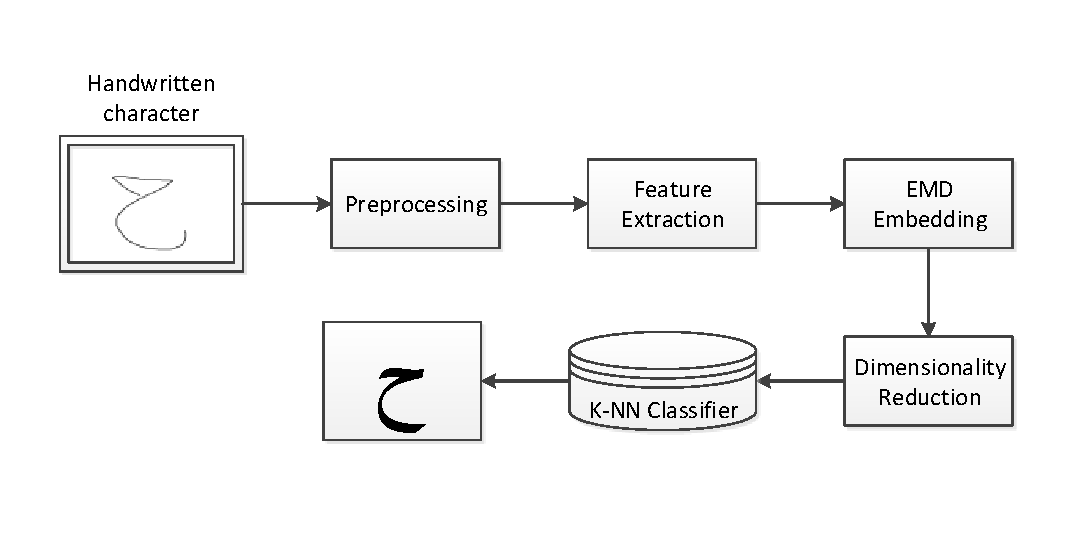
\includegraphics[width=1\columnwidth]{./figures/letters_classifier_learning_flow}       
\caption{High level diagram of the classifier learning flow for a letter position.}
\label{fig:letters_classifier_learning_flow}
\end{figure}
 
\subsection{Preprocessing}
Digitizers tend to generate a jagged and non-uniform sampling of the trajectory scribed on their surface.
This noise consists mainly of redundant successive points duplication and inadequacies caused by hand vibrations. 
In order to overcome the flaws mentioned, preprocessing operations are usually needed to impose certain uniform structure on the data, to comply with the input structure required for the proper operation of the subsequent parts of the system \cite{al2011online}. 
In the current work, preprocessing consists of three methods: \emph{normalization}, \emph{noise elimination} and then \emph{re-sampling}.

Size normalization is performed to achieve a uniform size of the bounding box surrounding the pattern. 
It was applied on each stroke so that it will fit into a $[0,1]\times[0,1]$ bounding box without affecting the original aspect ratio. 

Then, the \emph{Douglas-Peucker Polyline Simplification algorithm} \cite{douglas1973algorithms} was employed for eliminating such deficiencies in the data. 
It reduces the number of vertices in a piecewise linear curve, given a preset tolerance parameter $\varepsilon$, which defines the maximum 'dissimilarity' between the original and the reduced curve, and outputs a simplified curve, that consists of a subset of the points that defined the original curve.
In this work the tolerance parameter $\varepsilon$ was empirically set to ${1 \over 75}$.

The simplification process produces a highly angular, and non-uniform distribution of points along the stroke trajectory.
This stage, using splines interpolation method, aims to produce an equidistant smoothed data sequence, given a re-sampling target number of points $R$, which was set to 40. 
Given a stroke $S=\{(x_i,y_i)\}_{i=1}^{n}$, let $f_{x}(d)$ and $f_{y}(d)$ be the quadratic piecewise interpolations function of $\{x_i\}_{i=1}^{n}$ and $\{y_i\}_{i=1}^{n}$, respectively. 
$f_{x}(d)$ and $f_{y}(d)$ are functions of the coordinate value with respect to the arc-length distance from the pattern's starting point. 
Let $t_i=i\frac{L}{R}$ for $i=0,...,R$ where L is the arc-length of the pattern.
The re-sampled sequence is given as follows:
\begin{equation}
\widehat{S}=\{(f_x(t_i),f_y(t_i))\}_{i=1}^{R}
\end{equation}

Figure \ref{fig:before_after_preprocessing} show the resulting sequence after applying the preprocessing method on a sequence of the letter \RL{b}. 

\begin{figure}
	\centering
        \subfloat[]{
            \label{fig:preprocessing_orig}
            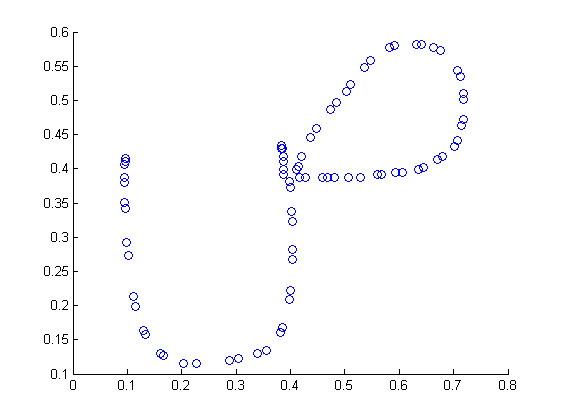
\includegraphics[width=0.4\columnwidth]{./figures/preprocessing_orig}
        }
        \subfloat[]{
           \label{fig:preprocessing_norm}
           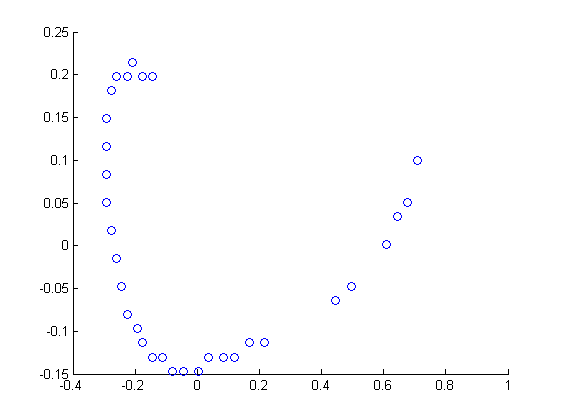
\includegraphics[width=0.4\columnwidth]{./figures/preprocessing_norm}
        }  \\
        \subfloat[]{
            \label{fig:preprocessing_simpl}
            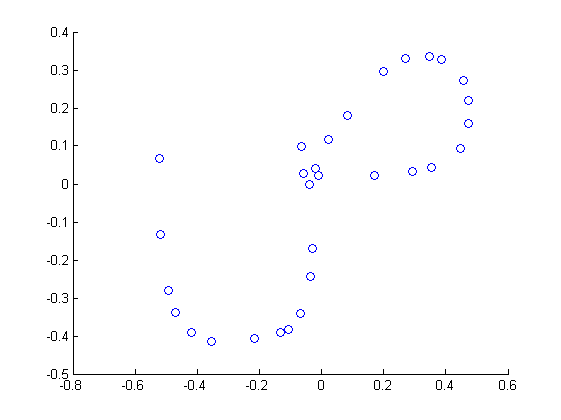
\includegraphics[width=0.4\columnwidth]{./figures/preprocessing_simpl}
        }
        \subfloat[]{
           \label{fig:preprocessing_resamp}
           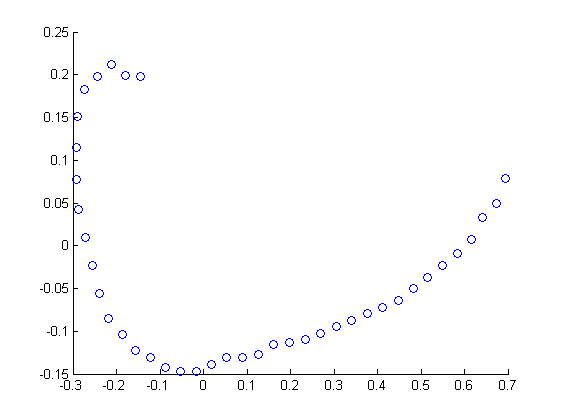
\includegraphics[width=0.4\columnwidth]{./figures/preprocessing_resamp}
        }       
    \caption{A sample of the letter \RL{b} before preprocessing (a); after normalization (b); after noise elimination (c) and after re-sampling (d).}
   \label{fig:before_after_preprocessing}
\end{figure}

\subsection{Feature Extraction}
In this work we have chosen to work with two shape descriptors, the \emph{Shape Context} (SC) \cite{belongie2002shape} and the Multi-Angular descriptor (MAD) that was proposed by Saabni in \cite{saabni2013multi}.

\subsection{The Earth Mover's Distance Embedding}
Histogram based descriptors, such as the Shape Context, are in many cases compared using a bin-wise dissimilarity techniques such as the Minkowski distance or the $\chi^2$ statistic.
Bin-wise dissimilarity measures can be computed very fast due to the fact that they measure dissimilarities between the content of corresponding bins of the two histograms and discard information across bins. 
Thus, they usually fail to consider local and global variations. 
These variations, which would be perceived as minor by a human, may result in a large dissimilarity values between two histograms. 

Generally speaking, the distance between two histograms can be viewed as a special case of the well-known \emph{transportation problem}, a.k.a the Monge-Kantorovich problem \cite{rachev1985monge}.
The \emph{Earth Mover's Distance} (EMD), introduced by Rubner et al. in \cite{rubner2000earth}, is a solution to the transportation problem which can be used as a measure of the dissimilarity between histograms. 

{Intuitively, given two distributions, one can be seen as piles of sand and the other as a collection of holes. 
The EMD measures the least word needed to fill the holes with the sand, where a unit of work corresponds to the transporting a unit of sand from one pile to the hole depending of their distance.}
EMD was experimentally verified to capture well the perceptual notion of a difference between images and is commonly used in content-based image retrieval to compute distances between the color histograms of two digital images \cite{grauman2004fast}.

The major hurdle in using EMD is its $O\left( {{N^3}\log N} \right)$ computational complexity (for an $N$-bin histogram). The complexity is magnified when the task is to search for similar shapes (nearest neighbours) in a large database. 
In this case, a linear scan of the database would require computing a comparison of super-polynomial complexity for each database member against the query shape \cite{grauman2004fast}. 
Greatly reducing the EMD calculation time can be achieved using approximation technique.  

Several approximation algorithms have been proposed to speed-up the computation of EMD. 
Indyk and Thaper \cite{indyk2003fast} proposed a technique for embedding the un-normed EMD metric into the $L_1$ space so that the EMD distance between the two objects is comparable to the Manhattan distance between the two points which represent the embedding of the two objects.
In a subsequent work done by Shirdhonkar and Jacobs \cite{shirdhonkar2008approximate}, the authors proposed a method for approximating the EMD between two low dimensional histograms using the weighted wavelet coefficients of the difference histogram. 
The approximation is done by transforming the histograms into the $L_1$ space so that the distance between the two vectors in the wavelet domain is the EMD approximation. 
Shirdhonkar and Jacobs showed that the embedding of the difference histogram approximates the EMD between two histograms. It is done by calculating the $L_1$ norm of the coefficients vector of the embedding as given in Equation \ref{eq:emd_embedding}.
\begin{equation}
d(p)_{wemd}= \sum\limits_{\lambda} 2^{-j(1+n/2)}|p_{\lambda}|
\label{eq:emd_embedding}
\end{equation}
where $p$ is the n-dimensional difference histogram and $p_{\lambda}$ is the wavelet transform coefficients. 
The index $\lambda$ includes both shifts and the scale j.
Intuitively, the wavelet transform splits up the difference histogram according to scale and location where each coefficient represents the solution to the EMD subproblem. 
For a single wavelet, the mass to be moved is proportional to the volume of $|\psi_j(x)|$, i.e., to $2^{-jn/2}$ and the distance to be travelled is proportional to the span of the wavelet, i.e $2^{-j}$. The sum of all distances is an approximation to EMD, as formally defined in Equation \ref{eq:emd_embedding}. 
This can be viewed as similar to the way packages are shipped over large distances. 
The route is broken into several pieces which are large and small distances. 
Packages from nearby places are merged at the end of the short distance route piece to travel together. 
Then another merge is done of packages from the entire country to be shipped together to the destination country. 
The sum of the distances travelled is an approximation to the actual distance.

However, in our application, where the histogram descriptors are to be stored rather than the difference histogram, the computation of EMD can be partitioned into two parts. 
First the histograms are converted into the wavelet domain and their coefficients are scaled according to Equation \ref{eq:emd_embedding}. 
Computing the EMD distance, in the next step, is done by calculating the Manhattan distance between the scaled coefficients of the corresponding histograms.
They provided both theoretical and experimental bounds. 

\subsection{Dimensionality Reduction}

The undesired properties of \cite{van2009dimensionality}, thus dimensionality Reduction methods are usually used for reducing the number of variables taken into consideration since  high-dimensional data present many mathematical challenges and practical complications. 
Ideally, the reduced representation should have a dimensionality that corresponds to the intrinsic dimensionality of the data \cite{van2009dimensionality} which is the minimum number of parameters needed to account for the observed properties of the data.
The need for employing dimensionality reduction in this work emerged from the sparse vectors produces by the EMD embedding of the feature vectors into the wavelet coefficient domain which produced vectors in $R^{3946}$. 
The wish to employ k-d trees, which is very sensitive to high dimensional data, was the main reason for using dimensionality reduction. 

In this work we have used a technique of applying \emph{principle component analysis} (PCA) followed \emph{linear discrimination analysis} (LDA) in order to obtain linearly discriminative information.
PCA is unsupervised in the sense that the labelling of the data do not effect the determination of the transformation function. 
It transforms the data to a new coordinate system such that the greatest variance by any projection of the data comes to lie on the first coordinate (the first principal component), the second greatest variance on the second coordinate, and so on.
As aforementioned, the target number of dimensions of the PCA step were determined according to the data preservation rate parameter which was preset to $E=0.99$. 
This can be calculated easily using the eigenvalues of the covariance matrix

The major drawback of PCA is that it is an unsupervised technique and as such does not use label information of the data
which may cause ...

LDA, a descendant of the original Fisher-LDA that was proposed by Fisher in \cite{fisher1936use}, overcomes this problem. Unlike PCA, LDA is a supervised technique. 
%LDA performs dimensionality reduction while preserving as much of the class discriminatory information as possible. 
%LDA has three main drawbacks; the first is that it assumes that the data resides in $L_2$; second, LDA assumes that the distribution of the samples in each class is Gaussian which is not necessarily true for our samples; third, it is much slower to calculate compared to PCA.
%Even though LDA is preferred in many application, it does not always outperform PCA. 
%In order to optimize discrimination performance in a more generative way, a hybrid dimension reduction model combining PCA and LDA is used in this work.
%
%The basic form of PCA is defined over the $L_2$ space. 
%However, the data that is embedded to the wavelet domain was proved to approximate EMD in the $L_1$ space. 
%Although $L_1$-PCA techniques were examined in the literature \cite{kwak2008principal}, we decided to use the basic form of PCA, given that $L_2$ estimate $L_1$ fairly well.

In the proposed system, we wanted to exploit the strengthens of both PCA and LDA techniques using the dimensionality reduction process which is outlined as follows: The samples are projected to a subspace $S_1$ using PCA and then to subspace $S_2$ using LDA. In the PCA stage, the target dimensionality, i.e., the number of principal components taken into consideration, is the minimal to achieve data preservation rate of 99\%, i.e., $E=0.99$. As mentioned before, the dimensionality of the original vectors was 3946. The reason we adopted such a high rate is that it was enough to secure a major dimensionality reduction. As seen in table \ref{table:dr_dimensions_results}, the dimensionality was reduced by PCA in two orders of magnitude.

Applying LDA directly on the resulted data would have achieved poorer results for the reason that almost all letters in the Arabic writing system have several shapes which are commonly used. 
Furthermore, since LDA regards the labeling of the data samples, trying to group different perceptual shapes in a single class would impinge the dimensionality reduction process. 
In order to overcome this obstacle, we have done the following preprocessing steps: each class was was partitioned into four clusters using $L_1$-k-medoids algorithm and received a different class label, and only then LDA was applied.

\emph{Intrinsic dimensionality estimation} methods are traditional techniques for estimating the intrinsic dimensionality of a data. 
The function that estimates this relation for a given data point $x_i$ is named \emph{local estimator}.
The estimated intrinsic dimensionality $\hat{d}$ of the dataset is then calculated by averaging over the local estimators of the entire sample set \cite{van2007introduction}.
The dimensionality of the data samples is shown in Figure \ref{table:dr_dimensions_results} for every database. 

\begin{table}
\centering
\begin{tabular}{ | c | c | c | c |}
\hline
Letter position & Number of samples & PCA & PCA+LDA\\
\hline                 
  Iso & 1372 & 29 & 7 \\ 
  \hline
  Ini & 1405 & 39 & 9 \\ 
  \hline
  Mid & 1196 & 36 & 8 \\ 
  \hline
  Fin & 1629 & 27 & 7 \\ 
  \hline
\end{tabular}
\caption{Dimensionality Reduction results.The original data set dimensionality is 3946. The PCA column shows dimensionality of the data after applying PCA. The PCA+LDA column shows the dimensionality of the data after applying LDA subsequently after LDA as described.}
\label{table:dr_dimensions_results} 
\end{table}

\subsection{Fast k-nearest Neighbour approximation}
In order to speedup queries, index structures are usually built over the sample set. 
The main goal of an index method is to enable efficient retrieval and similarity search, either asymptotically or simply in real wall-clock time. 
It aims at solving the problem of searching $k$-NN in a large set of multi-dimensional points by first building a data structure based on the set of reference points. Then, given a query object, it extracts the $k$-NN using this structure.
The time cost involved in building the index is amortized over the series of queries, and is usually ignored when considering search cost \cite{hetland2009basic}.

ANN methods such as k-d trees \cite{bentley1975multidimensional}, and Locality Sensitive Hashing (LSH) \cite{gionis1999similarity} have been successfully applied on a variety of fast similarity retrieval problems. 
k-d tree, a special case of binary space partitioning trees, is a data structure for storing a finite set of points from a $k$-dimensional space. 
However, the key assumption in these procedures is that the objects in the dataset lie in a metric space, i.e., the space satisfies the triangle equality, however, this assumption is not valid for many similarity measure techniques, such as EMD.
In the case of k-d tree, it requires the $L_p$ norm for its operation, which is even a more specific demand.
While the worst case scenario complexity is $O(N)$, the expected complexity of a single $k$-NN query using k-d tree is $O(\log N)$.

\subsection{Candidates Scoring}
For each subsequence, the recognition system returns a set of K potential letters candidates, with their resemblance scoring. 
In the current implementation we consider only the candidate with the best (minimal) scoring, however, any function taking into consideration the scoring returned by the classifier for all the candidate can be used to determine the final scoring of the cell.
Once the set of candidates determined by the closeness found by the k-d tree based on the coefficients vector in the $L_1$ space. The scoring is performed as follows:

The scoring of the candidates is done by averaging the score of the $L_1$ distance between the query object and the candidate in the sample set, and the score of the DTW distance between the feature vector and the 
Let us the denote the feature vector of the query object by $q$ and the feature vector the candidate $i$ by $c_i$.
\begin{equation}
Scoring(c_1)=\frac{EMD_{approx.}(q,c_i)+DTW(q,c_i)}{2} 
\end{equation}

This gives an equal weigth to the DTW and the EMD approximation.
We have found the constraint DTW performs using the unconstrained DTW.
The weights given for each similarity measure technique was determined empirically.

\emph{check other scoring techniques, such as DTW alone, EMD alone, DTW+Approximation}

\section{Samples Collection}
\label{sec:Samples_collection}
The ADAB database, described in \cite{el2009icdar}, is a de-facto standard in the field of on-line Arabic handwriting recognition. 
It is freely available and consists of more than 20k Arabic handwritten words (937 Tunisian town/village names) scribed by more than 170 different writers. 
Unfortunately, the ADAB only provides data on the strokes for a given city name. 
No segmentation into letters or \emph{word parts} (WPs) is provided by the database, thus, extra work was needed to add this information in order to use its letter samples and as a ground truth for the segmentation system.
To provide this information, we employed the skills of a human expert to segment the strokes into letters, and to determine the words and the WP boundaries for each sample. 
This additional information was saved in an XML file. 
Delayed strokes were not included in the processed information since it is not considered by the segmentation process.
We have manually segmented more than 7k samples which consisted about 20k strokes.
Using a public and not a self collected samples gives our results a further firmness.

\section{Results and Analysis}
\label{sec:results_analysis}

%\begin{enumerate}
%\item compare with other letter classifiers or digits.
%\item compare the performance of classification without using our approach.
%\item show the affect of the number of the sample set on the classification rate. If we show that the larger the sample set, the less is the recognition rate, it will contradict what wwe have said in the introduction about the need in a large training set.
%\end{enumerate}

The validation set, shown in Table \ref{table:sample_set}, was used for both training the system and testing the performance of the classifier.
Measuring the system accuracy and performance in all the experiments below were done using 10-fold cross-validation for each position letter database (Ini, Mid, Fin and Iso) independently.
The values calculated for the accuracy measures in the following experiments are done by weighted average of the performance of each position.

\emph{notes: remove the table. mention it in the text.}
\begin{table}
\centering
\begin{tabular}{ | c | c | c | c |}
\hline                 
  Ini & Mid & Fin & Iso \\ 
  \hline
  1404 & 1195 & 1628 & 1371 \\
  \hline
\end{tabular}
\caption{Sample size and distribution}
\label{table:sample_set} 
\end{table}

The results shown in table \ref{table:features_comparison} compares the two feature extraction techniques used in this work and compare it to the results obtained when none is used, namely, using the letter sequence as the vectors in the feature space.
It can be seen that the Sequence, i.e. using no feature extraction, have achieved almost the same accuracy results as when using SC.
Although at first glance it can make doubting the necessity the feature extraction stage, we will see in later that the use of SC improved the segmentation results considerably when performing the on-line segmentation and recognition.
It boosted the SR from 75\% to 81\% and the RR from 72\% to 76\%.
This may be explained by the fact that although the same accuracy results in letters classification, the scoring given to candidates is more accurate.


\emph{notes: Try to tune the MAD or else drop it.}
\begin{table}
\centering
\begin{tabular}{ | c | c | c | c | c |}
\hline
Feature & Precision & Recall & F-measure \\
\hline                 
  Sequence  (None) &  0.87 & 0.87 & 0.867 \\
  \hline
  Shape Context & 0.86 & 0.86 & 0.86 \\
  \hline
  MAD & 0.77 & 0.78 & 0.77 \\
  \hline
\end{tabular}
\caption{Features comparison. }
\label{table:features_comparison} 
\end{table}

The next series of experiments aims to quantifying the contribution and importance of each stage in the classification required us to conduct a series of experiments.
In each experiment, we skip a stage in the recognition system and then measure the classifier performance.
The three main stages in the classifier are: 1. the feature extraction stage; 2. the EMD embedding; and 3. the Dimensionality reduction.
As detailed in Section \ref{sec:dr} the role of the DR process is to reduce the number of variables taken into consideration by the classifier in order to avoid problem caused by the "curse of dimensionality", without affecting much the system accuracy.
Table \ref{table:dr_embedding_comparison} shows the results of the experiment that uses SC as the feature.
The results in Table \ref{table:dr_embedding_comparison} shows that the dimensionality reduction technique implemented in this work almost does not affect the system performance.


\begin{table}
\centering
\begin{tabular}{ | c | c | c | c | c | c |}
  \hline
  Experiment & Precision & Recall & F-measure\\
  \hline                 
  Baseline &  0.87 & 0.87 & 0.867 \\
  \hline
  No DR & 0.91 & 0.9 & 0.90 \\
  \hline
  No embedding & 0.89 & 0.89 & 0.89 \\
  \hline
\end{tabular}
\caption{Different Experiments}
\label{table:dr_embedding_comparison} 
\end{table}

\subsubsection{Sample set size and distribution}
The letters is our training set are extracted from a database with a limited words diversity, thus, the distribution of the samples between the different classes is imbalanced. 
On one hand, it can be regarded as an advantage; since, the training set distribution reflects the a-priory probability of a letter appearance in the test set. 
On the other hand, a highly imbalanced training set is known to negatively affect many classification algorithms.
In the following experiment, we measure the effect of a large and imbalanced training set on the WP segmentation and recognition rates. 
It is done by gradually increasing the maximal allowed number of samples per class (letter and position).
 
The graph in Figure \ref{fig:num_letter_impact} shows convergence of the system's performance when the maximal number of samples is larger than 200 per class. 
Nevertheless, a miniature degradation is apparent, which is caused, probably, due to the increasing imbalance in the distribution of the training set.
In addition, it is evident that the recognition rate (RR) is more sensitive to small training set than the segmentation rate (SR).

\section{Summary and Future Work}

\section*{Acknowledgment}
The authors would like to thank Professor Dana Ron, from the Tel-Aviv University, for her invaluable help in this research and her insightful comments on this paper. This work has been supported in part by the German Research Foundation under grant no. FI 1494/3-2.

\bibliographystyle{IEEEtran}
\bibliography{IEEEabrv,bibliography}

\end{document}


